\chapter{Design}

This chapter describes the design rationale in relation the current system. This chapter will cover the overall system archtiecture, user interface designs as well psuedo code reprsentations of the main, non-trivial algorithms.

\label{DesignSec}
Section \ref{processSec} states how the author has a somewhat flexible approach allowing for adaptations to the initial design stated in appendix B. This section explores how the process has enabled the significant change of design to be implemented easily and without severe complication. The proposed design in appendix B and the final structure of the system are very different however, at an abstract level the key components still exist they are just represented different in each system architecture. 

\section{Language}

The author has identified that the choice of language is an essential decision which must be made early in the projects development cycle. Appendix B, section \ref{lang} denotes the language decision process the author went through and ultimately states the final language choice.

The use of an appropriate language became even more important due to the fact that the design has undergone significant modifications since the initial proposed design. If the author had selected a language which happened to be unfamiliar but seemed good at the time, then the changes made to the initial design may have been much more complicated to implement. The author is very familiar with Java, more specifically Java 7 (Java 1.7) and above thus, implementing new features or refactoring existing systems is fairly familiar territory. The initial language choice rationale (appendix B, section \ref{lang}) did not factor in the potential for radical design change however, if it did the outcome would not change and the existing rationale would still be applicable to the project. In the authors opinion Java is the most appropriate language for this project.

\section{Development Tools}
\subsection{Development Enviroment}

\subsubsection{Command Line Tools}
\label{sseccmd}
The author considered using the combination of a simple text editor which in this case would have been Atom\cite{atom:textEditor} to write the code, and compilation of such written code using the command line and the default complier through the use of the $javac$ command. Atom is a free, open source hackable text editor provided by GitHub and provides syntax highlighting support for numerous language, including Java which is the language of choice for this project. This syntax highlighting is especially useful and makes the writing of the source code slightly easier, as is becomes much simpler to track the start and termination points for specific code blocks. However, as Atom does not have built in Java compilation abilities, the compilation process can become somewhat complicated.

Using this approach, the Java source files composed using Atom must be complied using the default Java complier, provided by the language specification. The problem with this method of compilation is that error detection and correction can become a very tedious process. If any complication errors are present after the $javac$ command has been executed, the trace presented in the terminal window can sometimes be quite difficult to parse for the error message, and tracking down the error in the source files could be a difficult task. For smaller projects, this method of complication is perfectly suitable and can be effectively managed. However, this project as discussed in section \ref{processSec} this is a rather large project for the author to undertake. As this is the case, the combination of size of the applications source code and manual complication leads the author to believe this method of writing and compiling code is not only inefficient, but also inappropriate for this project and could potentially hinder development.

\subsubsection{Intergrated Development Environment}

The use of an Integrated Development Environment (IDE) can help to alleviate the problems that can come from using a writing and complication process such as that defined in section \ref{sseccmd}. There are many IDE's which support Java, however the author has preference is the use of the Eclipse IDE for Java Developers \cite{eclipse:IDE}. The Eclipse IDE provides a multitude of useful features as part of their default package. 

One of the main features which Eclipse provides is automatic building of the probjects source. This is a major benefit when developing as you can simply write your code and run the built project without having the unnecessary complication of switching between several applications to achieve the same task. Also, as there is automatic building, any compilation errors will be clearly highlighted using a system which is familiar to most computer users. If there are any miss-spellings of method or variables names for example, Eclipse will underline these in red to show there is a clear problem with this exact line of code. This is similar to the default scheme provided by most word processors, enabling a logical mapping between this red underlined line of code and the fact that there is an error present there.

Another useful feature provided by the Eclipse IDE is the auto completion of variables and method names. This has sped up the development process for the author as there was no need to constantly look at the API's or other project source files for method names, the author could simply type the Object of interest's identifier and see a list of all methods and variables associated with such Object. This is not possible to do if the author used an approach similar to that discussed in section \ref{sseccmd}.

In addition to the built in compilation feature, Eclipse also provides an integrated debugging toolkit. The Eclipse debugger enables easy creation and removal of break points, as well as all the usual features you would expect from a debugger such as, step through and step over, exploring the various contents of different variables and objects. These features are also provided by command line debugging tools, however the author is far more comfortable using a graphical interface to debug the application as it is much earlier to access the features of the debugger using this approach.

Eclipse also has built in Junit support. This project will use the JUnit library as part of the testing process (more details see \ref{junitsupport}). Similar to how the IDE makes the writing of the applications code easier, the support of test suites such as JUnit makes the test process much easier. The code responsible for the tests will also have access to the features provided by the IDE as mentioned above, this includes in place builds and auto completion. In addition to this you can run the tests inside the IDE and get accurate feedback on how many test ran, how many failed and why these tests failed. The author uses this to identify failed tests to be easily identified and repaired. Eclipse also supports a variety of other languages and features but these are not relevant to this project currently.

\subsection{Support Tools}

\subsubsection{Maven}

Maven is tool used for building and managing projects, specifically Java-based projects \cite{maven:site}. The Maven framework provides a lot of useful utilities for developing successful Java-based projects and ensuring that such projects adhere to certain standards. The Maven framework aims to provide convention, over configuration. If there are multiple projects which have many different dependencies, some of which could be external Jar files, then Maven can allow other projects to make use of these dependencies. As a result, if a new project is decided there is less time spent configuring as the dependencies are already presented using this Maven framework. However, the author is working alone, and is not expecting to have any other projects which will share dependencies with this one, thus the author has to weight up if this framework would actually help the development process.

Maven provides some useful testing capabilities. When testing using the Maven framework, tests are still written using the Junit libraries (see \ref{junitsupport}). However, the Maven framework provides some additional features which the author feels could be of use. Maven, will give the author a Unit test report should one be required which will cover numerous details, most important a coverage report will be produced. This enables the author to assess how well the unit testing has been done. Although this test report is a very useful feature, the Maven is not a necessity nor is it complication free.

The main complication that the author has with use the of Maven for this project is that fact that as this is generally a small project, Maven and its features would not be fully utilised but the hassle of configuring the framework would still be present. The initial project configuration would be time consuming, given that the author is inexperienced with the framework and this time could be spent on the actual project development. There are plugins which enable Maven to be used with an IDE such as Eclipse, the author feels that Maven would not be appropriate for use here, however the test reports would be extremely useful.

\subsection{GitHub}

The author has seen the use of GitHub as an essential part of the development process. GitHub has enabled the author have strict version control throughout the development process. As this is the case, the author has been able to store a local repository, which will exist as the working directory for the applications development whilst also allowing a working copy, with the current most up-to-date fully working project code to be stored safely online using GitHub. There has been numerous times throughout the development lifecycle where the author has had to revert back to a previous version of the applications code, GitHub has allowed this process to be more hassle free. As it is so simple to manage different versions of the application, each representing a different collection of working or non-working features the author has been able to develop in confidence as he knows that any mistakes or experiments are not very costly as there is always a backup version stored at the GitHub repository location.

Without the use of GitHub (or another version control system) the author would have found it difficult to progress the application as expected. If there was no form of version control, then the mistakes the author made or external factors which then rendered the current development code unusable would be a far more disastrous. There was a time during development where the authors working directory became corrupt. This was easily resolved by simply retrieving the code stored in the projects GitHub repository, however if GitHub was not being used here, then there would have been a high possibility than the author would have lost all progress on the application.

\subsubsection{JUnit}
\label{junitsupport}

JUnit is an open source framework for unit testing Java applications. The Junit libraries provide a multitude of features that allow for a more simplistic approach to testing. Numerous other test frameworks are available however, the author is very experience with JUnit and feels that the features provided by this framework are more than suitable for the unit testing of this application.

The author feels that a testing framework is essential for efficient and accurate unit tests for any application. If the author had neglected to use a testing framework such as Junit and manually tested the application using a looking manually for abnormal output (LMFAO) then the quality and coverage of the unit testing would reduce significantly. If the author used a manual approach such as this which relied on outputs then the author could potentially have a situation where the code in outputting the correct result, but the inner workings are expressing incorrect behaviours which can’t be manually checked. This means that you could ship a product which is assumed to be functioning as expected then suddenly, the application is significantly misbehaving. In addition to this it is difficult to automate manual testing as the author would need to check the outputs himself. A testing framework such as JUnit not only allows for the tests to be fully automated, the tests also become scalable. Every code change would need to be re-evaluated against the existing unit tests, which is easily done if you have a series of test which can be executed automatically. If a manual approach was used, then it becomes a near impossibility that every change can be tested as it would simply be too much to check as the addition of this new code has scaled the number of application inputs and outputs as well the conditions in the codes logic.

\section{Overall Architecture}

The process used during this applications development has enabled the author to modify the proposed overall architecture significantly. This has enabled the author to add additional features which were not additionally planned, this includes the addition of extra algorithm types and modifiers as well as enabling the potential heavy refactoring of code into more logical methods and classes. The new application architecture is much more complex that the initial proposed design, as a result each package will be represented as its own set of diagrams, and then an overall representation showing the interactions between these packages will be explained. In all figures below, getter and setter methods are emitted but are assumed to be present. The packages referebced in this section will take the form of $che16.dcs.aber.ac.uk.xxx$ where $xxx$ is the corresponding package name.

\subsection{Controller}

The Controller package has undergone several changes since the initial design of the system as defined in appendix B, section \ref{sssec:cntrl}. The general ideologies have however remained the same, the ranges of features provided by the application as a whole has increased thus, the author saw these modifications the Control package contents as a necessity in order correctly control these new features whilst also adhering to the existing Model-View-Controller framework.

\begin{figure}[H]
\centering
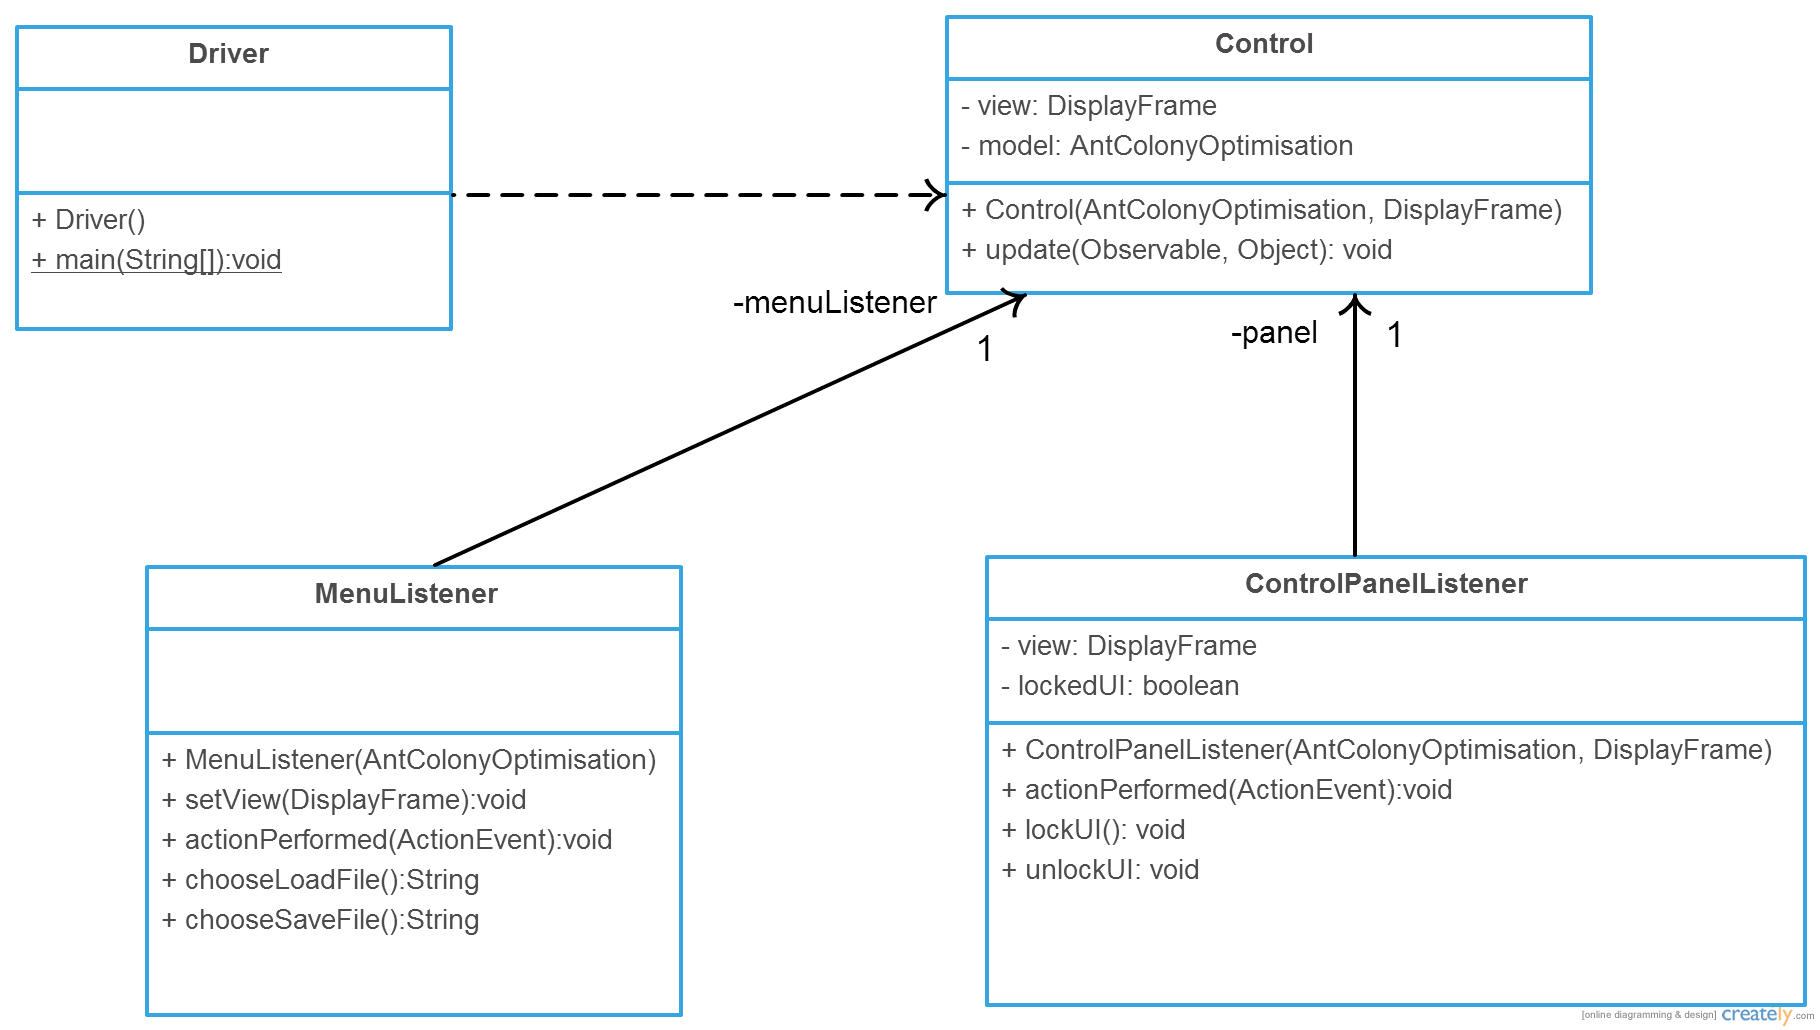
\includegraphics[scale=0.23]{Images/chapter4/controller}
\caption{The contents of the Control package show in standard UML Class diagram notation}
\label{fig:controllerImp}
\end{figure}

\subsubsection{Class Descriptions}

The \textbf{Driver} Class remains largely unchanged from its initial proposed design (see appendix B, section \ref{driver:classdef}) however, it now interacts with the other components in a slightly different manner. The Driver Class remains as the entry point for the application, however, the Driver has the additional responsibilities of instantiating the Control instance, as well as handling the correct associations needed. The general purpose of the Driver Class is still to ensure the system components are correctly instantiated, and holds no references to any instances of any Object.

The \textbf{Control} as represented in figure \ref{fig:observableImp} is designed to observe the model and notify the view should the state of the model change significantly. In addition to this, the required instanced of MenuListener and ControlPanelListener are instantiated in this Class, and a reference to this Control Object is maintained the created instances of said Objects. The Control Class is an additional feature not present in the initial design, this is because as represented in figure \ref{fig:observable} the DisplayFrame initially observed the model, this has since been modified. This Class has the potential to be extended to support several other Observable Objects should this functionality be needed by the author in the future.

An instance of the \textbf{MenuListener} is used to listen the JMenuBar present in the DisplayFrame. This is designed to enable a collective way to manage all actions represented by the items contained in the JMenuBar. The alternative approach is to give each element in the JMenuBar its own Action Listener. This is far from efficient and increases both the codes complexity, and reduces overall maintainability of the application. The author decided to use a dedicate Object such as this, to listen to the menu and perform appropriate actions. This Class maintains an instance of the Control Class, this enables the instance of this Class to have access to the model and view instances stored in the Control instance enabling a simple way for the JMenuBar to have access to necessary functions.

A \textbf{ControlPanelListener} instance is designed to be a dedicated ActionListener for the ControlPanel (see section \ref{model:classdef}) instance. Two separate ActionListeners are present in this application, this is because the author wanted to have dedicated listeners for each component, rather than having a combined Object representing this Class and the MenuListener Class. The author feels that this is appropriate as any behaviour modifications or changes the Object which will be listened to becomes much simpler to accomplish if relevant behaviours are extracted into logical modules such as this design exhibits.


\subsection{View}

The View package serves the same purpose as initial designed however, there has been a singnificant amount of refactoring applies to the initial design to enable a more effective graphical user interface to be created. The author has also added several new Classes into this package to represent additional views which were not initially visioned, but during development the author recognised that these new views were essential.

\clearpage
\begin{sidewaysfigure}
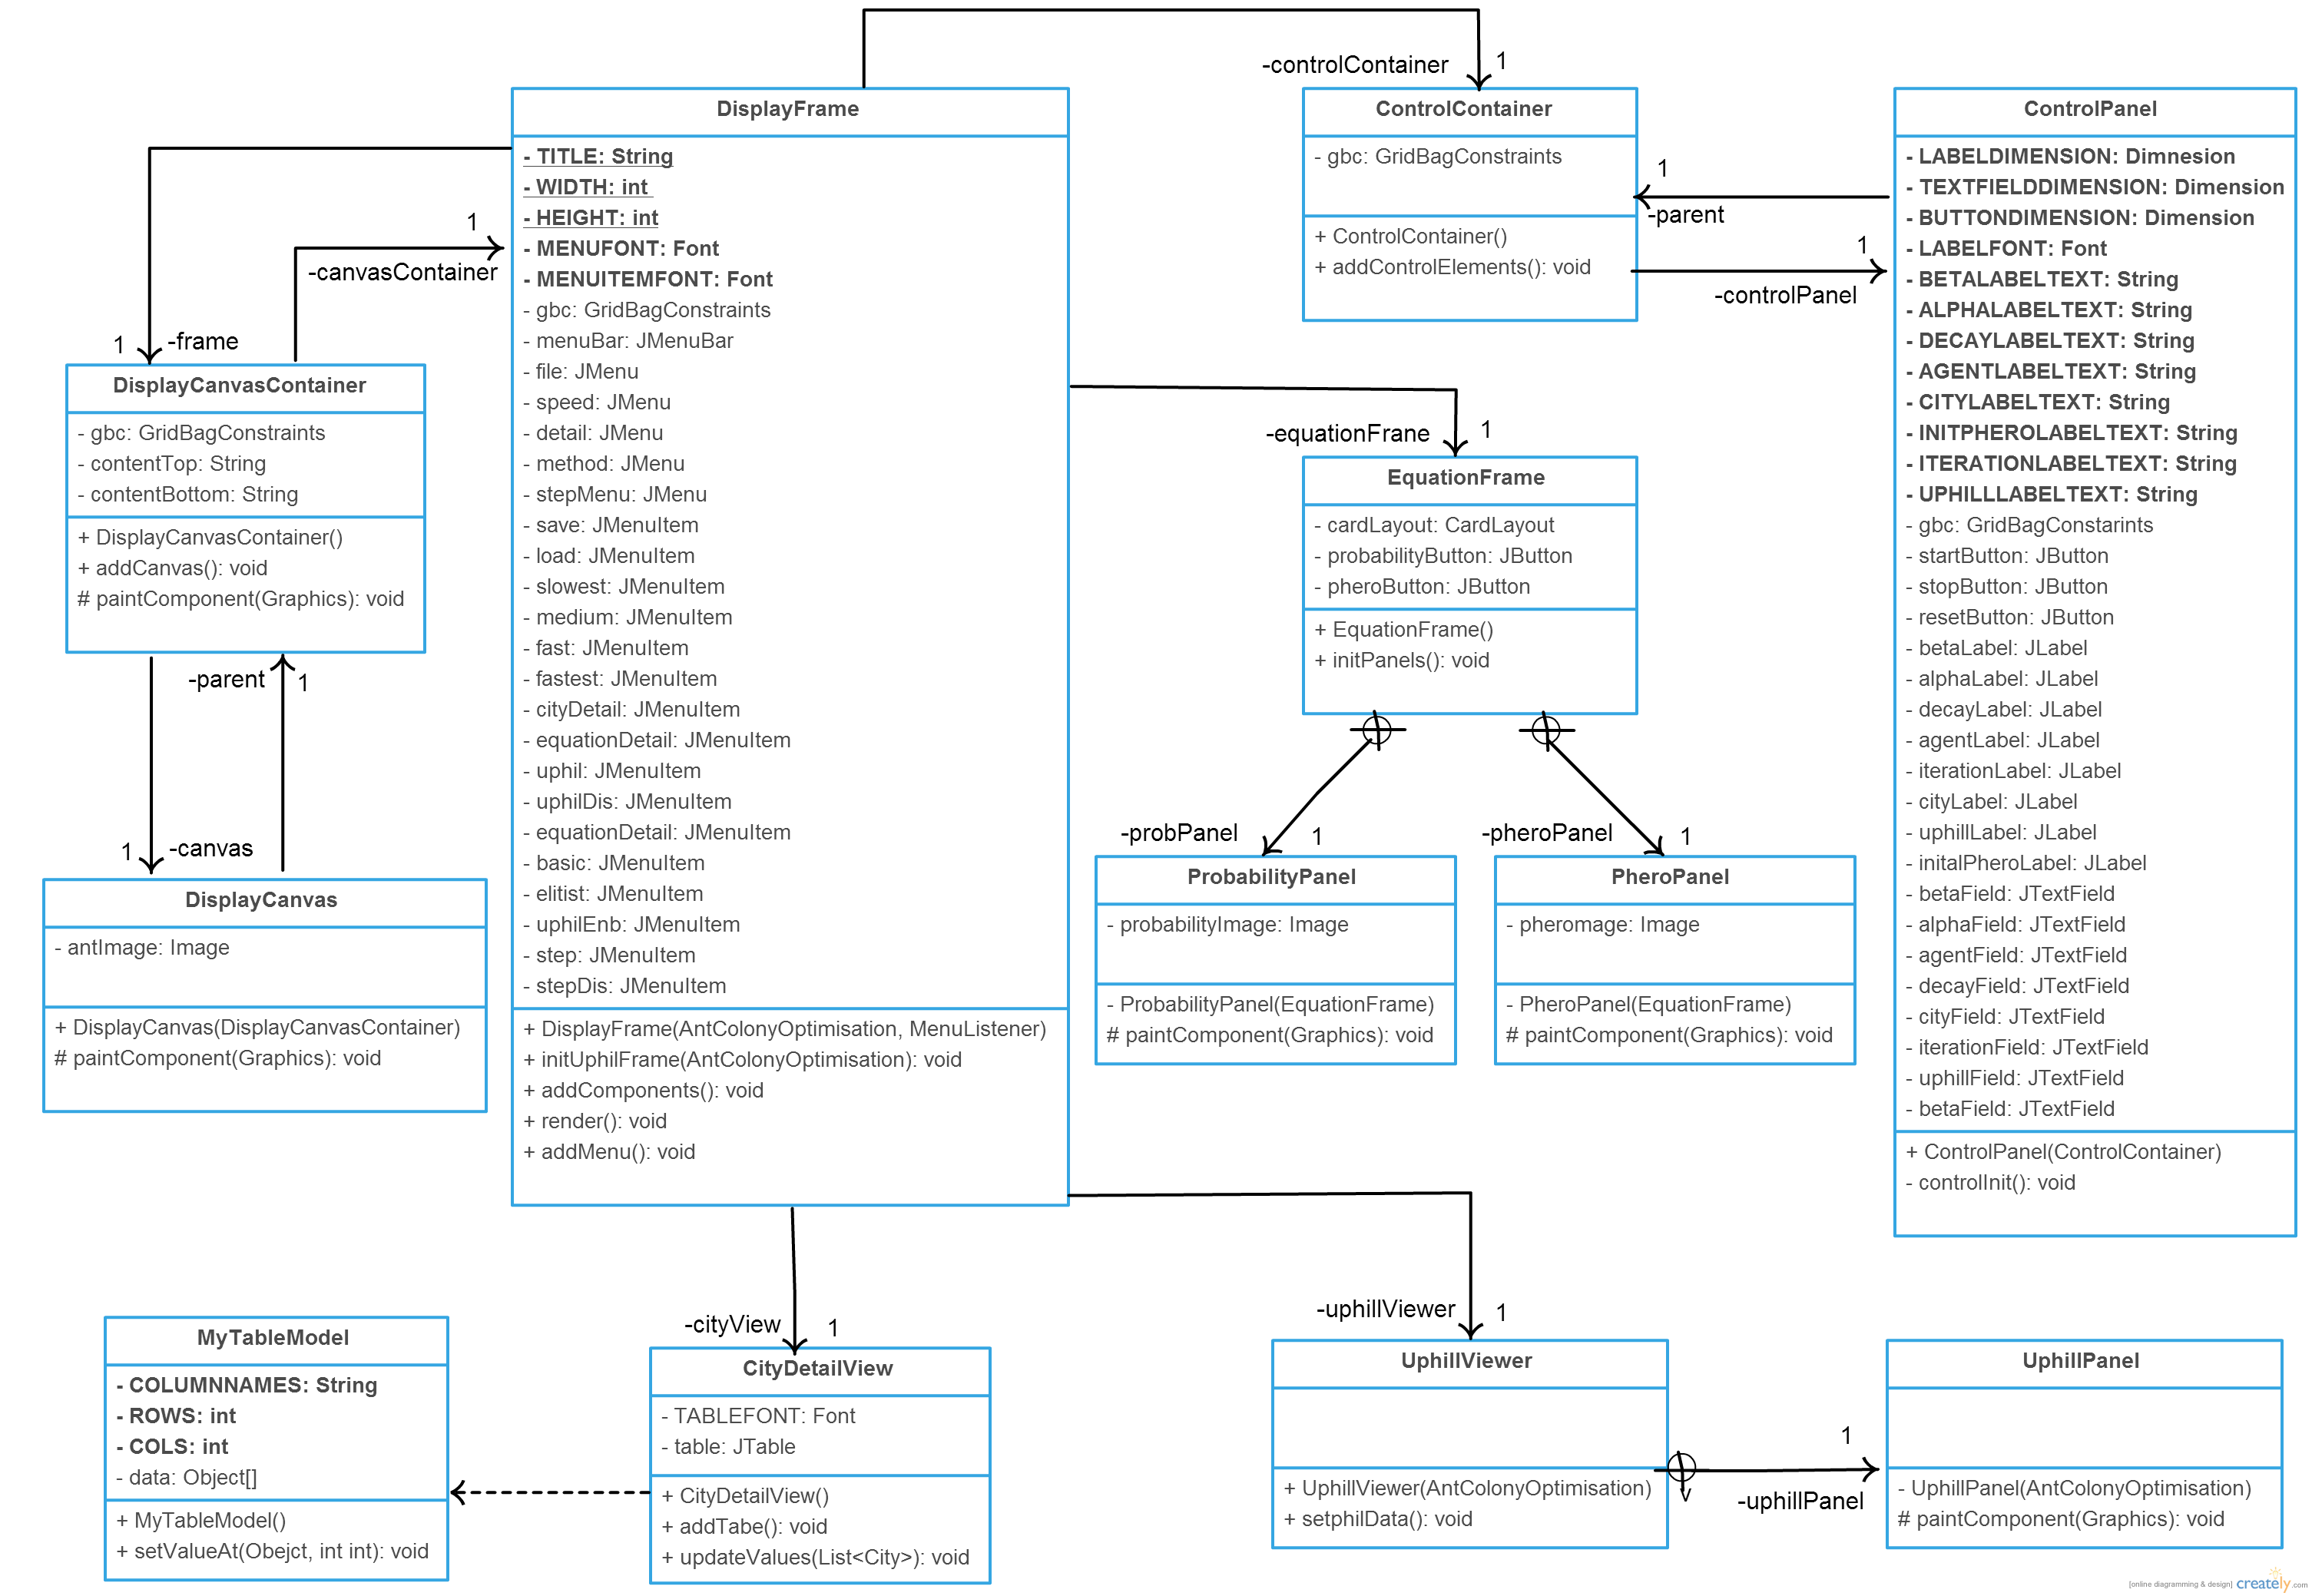
\includegraphics[scale=0.225]{Images/chapter4/view}
\caption{The contents of the View package show in standard UML Class diagram notation}
\label{fig:classdiagramImp}
\end{sidewaysfigure}
\clearpage

\subsubsection{Class Descriptions}
\label{view:clss}
Initial the \textbf{DisplayFrame} was designed to simply represent the highest level container which houses the remaining graphical user interface elements. As figure \ref{fig:classdiagram} in appendix B shows the initial design for this class happened to be very simplistic and lightweight. The author decided to include an additional user interface elements which was not originally planned. This addition happened to be JMenuBar, which was contained within this DisplayFrame instance. As this is the case, the DisplayFrame Class grew it size as it now encapsulates the JMenuBar and the menu elements of said JMenuBar as well as defining constants such as font styles. Although the size of this Class has grew, the complexity and functionality remains unchanged, it remains as the highest level container for the graphical user interface and control the instantiation of such elements.

The \textbf{DisplayCanvasContainer} is the result of renaming the DisplayPanel Class in the initial design (see Figure \ref{fig:classdiagram}, appendix B). This Class is designed as a container to the DisplayCanvas instance, this functionality is as designed and the author has not modified its behaviour.

An instance of the \textbf{DisplayCanvas} Class is used to actually visualise the algorithms state of execution to the application user. This will be the component that is painted during the algorithms execution using the $paintComponent$ method which it inherits from its JFrame super Class. As the functionality provided by this Class is very simplistic, the current implementation remains unchanged from the initial proposed design (see Figure \ref{fig:classdiagram}, appendix B).

The addition of the \textbf{CityDetailView} is a simple JFrame container which is used to display a JTable with data representing the number of agents currently at each city in the current World. The JFrame displayed by this Class can be toggled between visible and invisible through user interaction with the respective JMenuBar item.

The structure of the table represented visually by the CityDetailView, is modelled by the \textbf{MyTableModel} Class. Extracting the table’s structure into a separate Class enables easier modification of the structure as well as reducing the coupling between the view and the table itself.

Similar to the DisplayCanvasContainer Class, the \textbf{ControlContainer} Class is used to contain the user input elements in their own separate location. This is a result of refactoring the UserInputPanel Class in the initial design (see Figure \ref{fig:classdiagram}, appendix B) into this container and the ControlPanel Class. The main purpose for this Class is to allow more a more diverse range of positioning utilities to become available allowing for an easily modifiable interface.

The \textbf{ControlPanel} Class used to contain the interface elements which directly relate to the creation and modification of the problem and world. This includes housing the text fields and labels required to enable the user to customise the algorithm parameters, as well as providing a simple means to start and stop the execution using a simple JButton approach. This Class is essentially an extended version of the UserInputPanel Class in the initial design (see Figure \ref{fig:classdiagram}, appendix B), aside from the fact that more interface elements have been added, the functionality is the same.

The \textbf{EquationFrame} Class an extension of the JFrame Class which is used to display an graphic explaining the workings and functions of the underlying algorithms. As this is an educational application. The Class has no other functionality aside from the providing a means of displaying such graphics which is itself, contained within the ProbabilityPanel and PheroPanel Classes.

Both \textbf{ProbabilityPanel} and \textbf{PheroPanel} are nested Classes inside the EquationFrame Class. These Classes are extensions of the JPanel Class and are used to contain different graphics which will be used to represent information relevant to the underlying probability and pheromone functions respectively.

the \textbf{UphillViewer} Class is another new addition which was not perceived in the initial design. This Class is a sub Class of JFrame and is used to house an UphillPanel instance. This JFrame can be togged between visible and invisible with relevant user interaction with the JMenuBar contained in the DisplayFrame.

An instance of the \textbf{UphillPanel} Class is used to display information about the current status of the uphill routes for the current algorithms execution. This is an extension the JPanel Class, enabling the uphill route data to be painted to the component using the inherited $paintComponent$ method. This is a nested Class inside the UphillView Class as the author felt a this was the most appropriate way to represent such a Class  as no other Class uses or needs the knowledge of this Class.

\subsection{Model}

The elements contained in the initial proposed designed represented in  Figure \ref{fig:classdiagram}, appendix B have undergone significant refactoring which has produce a vastly different structure. During the development process the athour found the the intial design happened to be inaquate for representing the aglorithm in a suitable manner, as it lacked necessary components and detail.

\clearpage
\begin{sidewaysfigure}
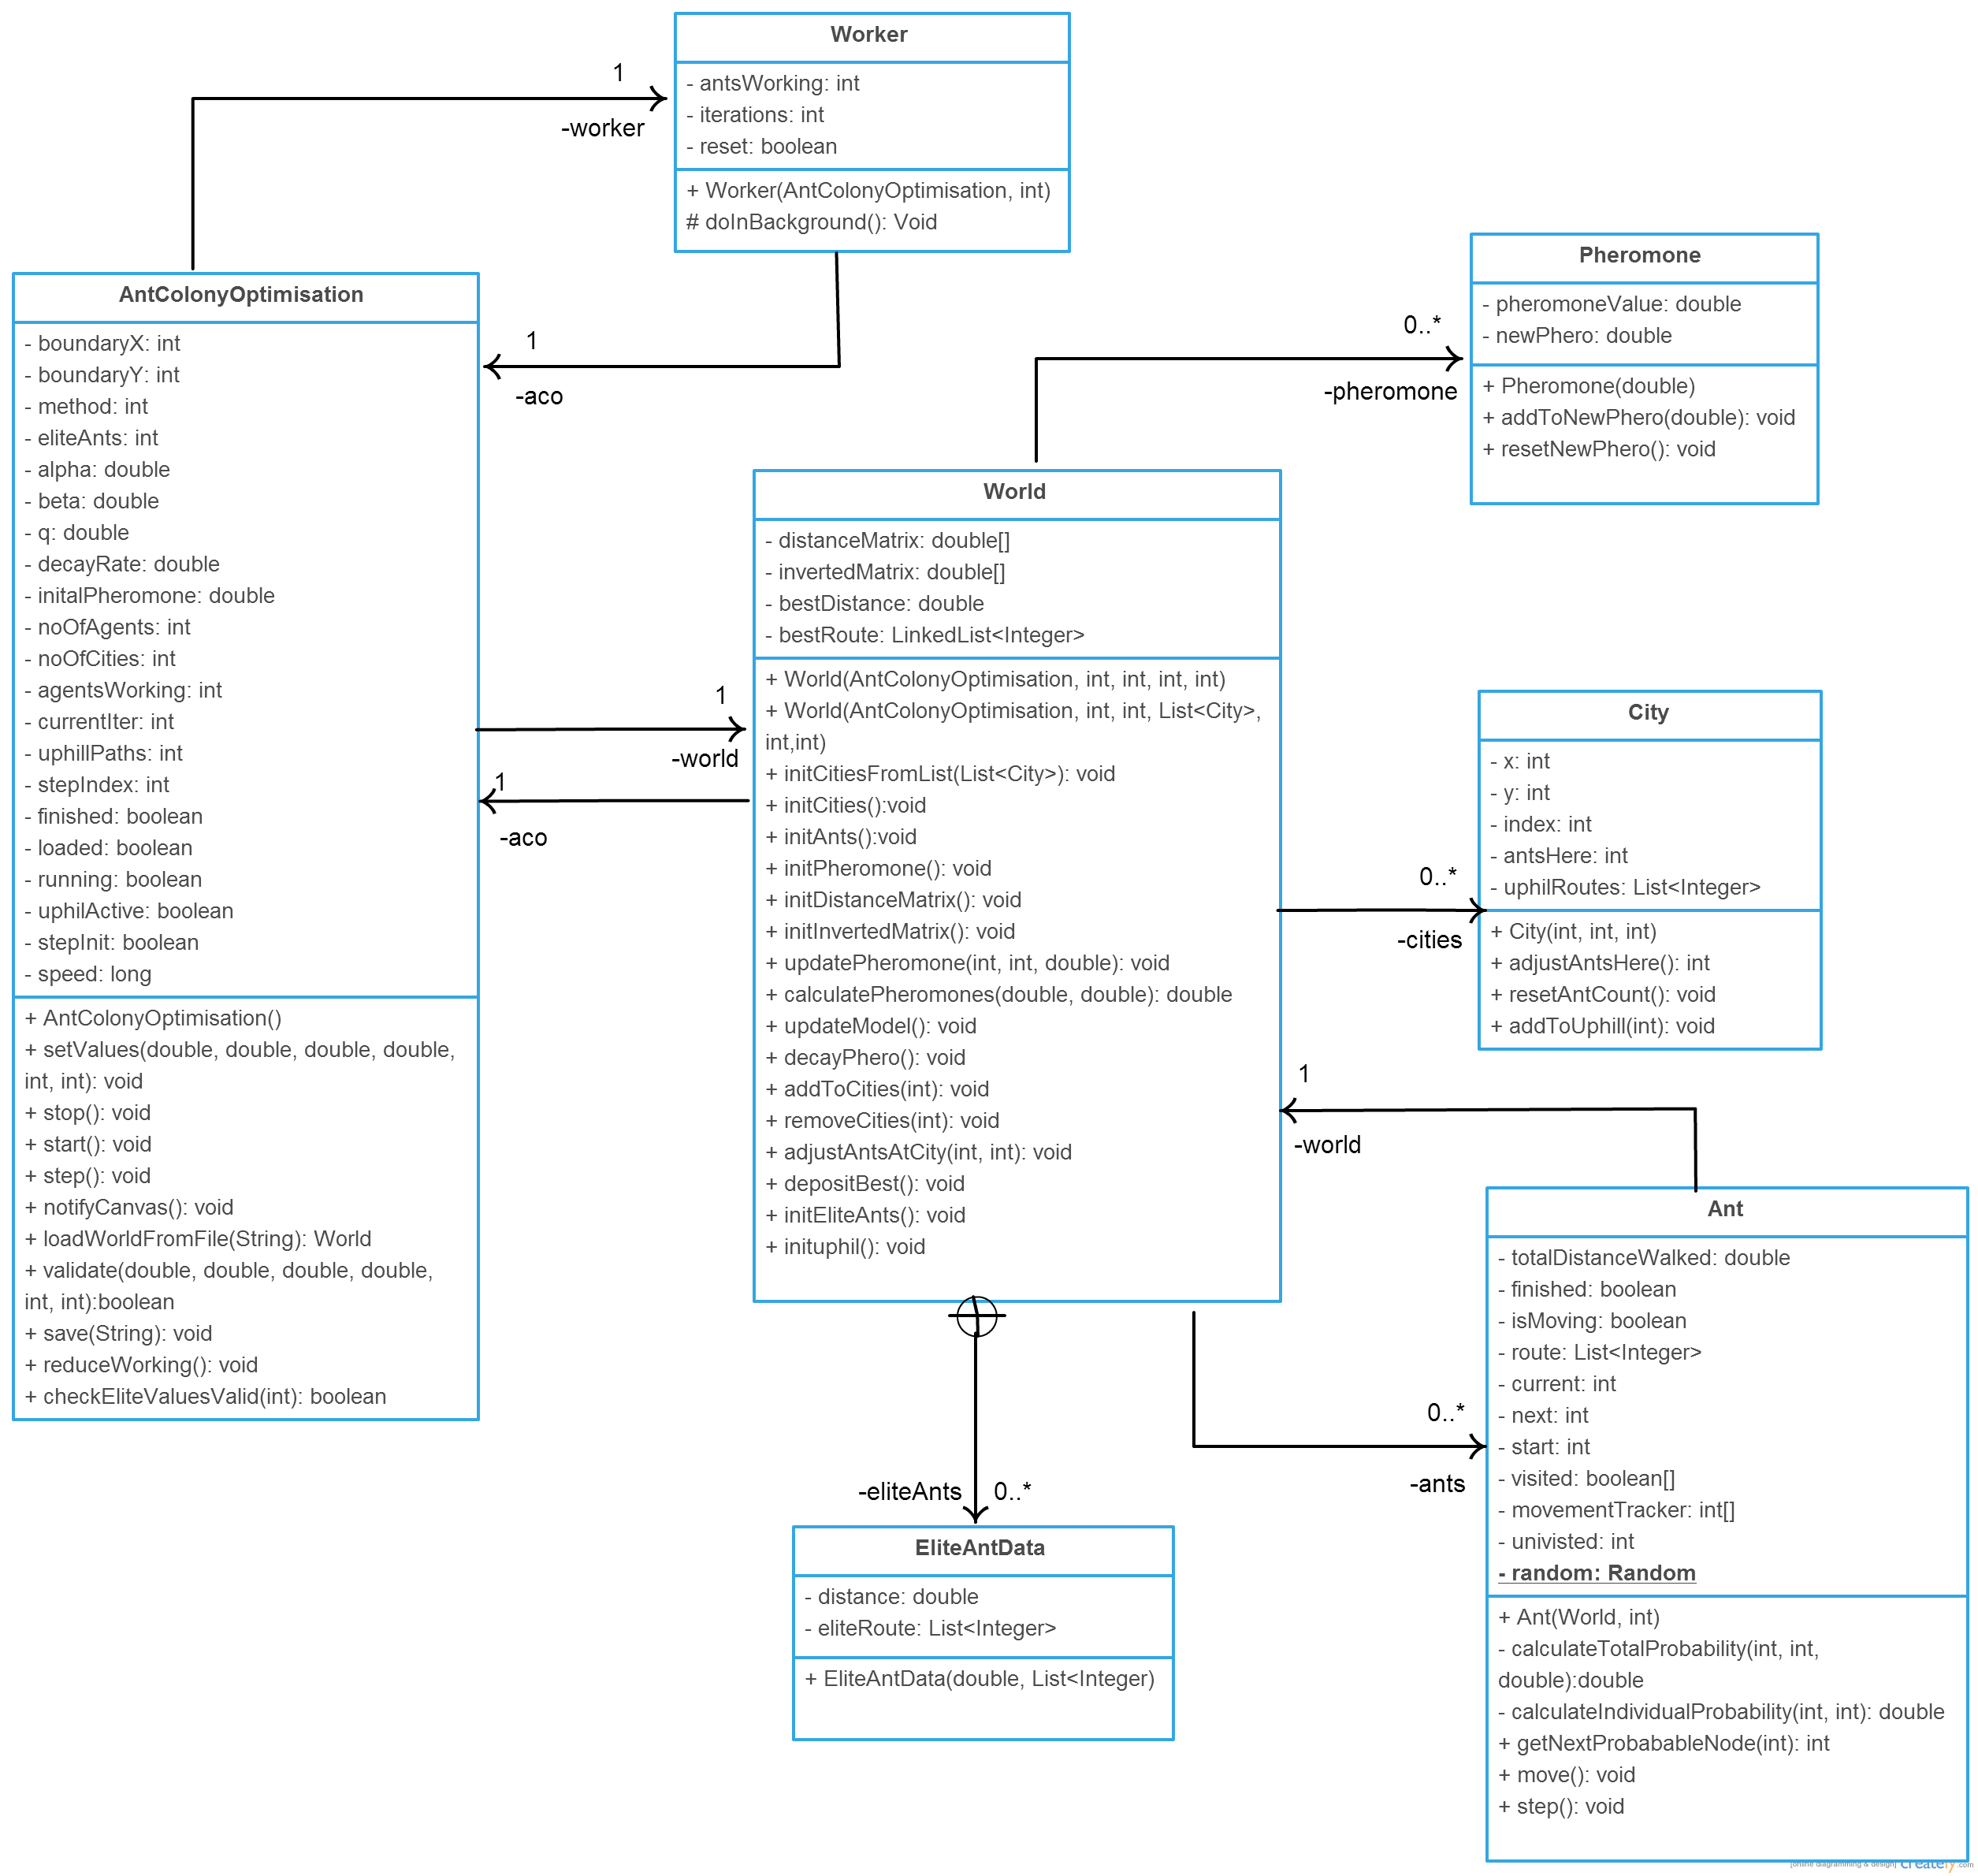
\includegraphics[scale=0.22]{Images/chapter4/model}
\caption{The contents of the Model package show in standard UML Class diagram notation}
\label{fig:classdiagramImp}
\end{sidewaysfigure}
\clearpage


\subsubsection{Class Descriptions}
\label{model:classdef}

The initial concept behind the \textbf{AntColonyOptimisation} Class is that this servers as the main control point and data centre for the algorithms representation. This Class is used to store all the necessary parameter values and is also responsible for in instantiation of the Word representation and therefore, indirectly the graph. This Class also controls external package access to the Model package and its data. This largely remains the same as designed, however, there are slight modification to accommodate the extra functionality added.

The \textbf{Worker} Class was something that wasn’t initially planned. As discussed in \Large REFERENCE IMPLEMENTATION OF SWING WORK \normalsize there was a necessity for a way to control the algorithms execution without interfering with the performance of the system or host machine. This Class is an extension of the SwingWorker Class and uses the inherited $doInBackground$ perform the algorithms execution in a suitable manner. 

The \textbf{World} Class is used to model the problem representation and the environment which the agents will be deployed during the algorithms execution. This Class houses all the data relevant to such representations including a List of all Ant and City Object as well as having basic data structures which provide an effective representation of the pheromone concentrations for every edge within the graph. This Class also handles the manipulation of pheromones on such edges. This Class is generally the same as proposed in Figure \ref{fig:classdiagram}, appendix B excluding the additional feature support.

A \textbf{City} Object is used to represent a node in the current problem representation graph. A list of these City Object is maintained in the current World instance, and iterated through during both the solving and painting processes.

A \textbf{Pheromone} Object is used to model the pheromone concentrations for any given edge. A two-dimensional array of these Objects is maintained in the current World instance, and these Objects are constantly manipulated during the pheromone deposit and decay operations. 

An \textbf{Ant} Object is used to represent an agent which will be deployed in the current environment in order to solve the current problem. The World instance will maintain a list of all current Ant Objects. Each Ant is able to move and deposit pheromone accordingly, this these Objects have sufficient variables and methods to enable this functionality. The initial design suggested the use of an AntInterface, however as the author has decided that there will only be one type of Ant Class, he has deemed the Interface to be unnecessary. Generally, this Class is as designed in Figure \ref{fig:classdiagram}, appendix B.

The \textbf{EliteAntData} is a nested Class inside the World Class which is used to store the current elite routes. This feature is only necessary if the user has selected ElitistAnts as the current algorithm type. This is required as if there are numerous iterations, the Ant Objects get reset each iteration and this is a lightweight way to store the elite ants for the course of the algorithm execution, as storing just the distances and routes of the best ants has less overheads when compared to storing whole Ant Objects.

\subsection{Utils}

During development the author decided that there were methods that were being repeated implemented in numerous places, in order to prevent code duplication and promote reusability the utils package was implemented. This is a very simple package, containing one Class, however, the contents of this Class don't belong in any other package individually thus, have been implemented separately.

\begin{figure}[H]
\centering
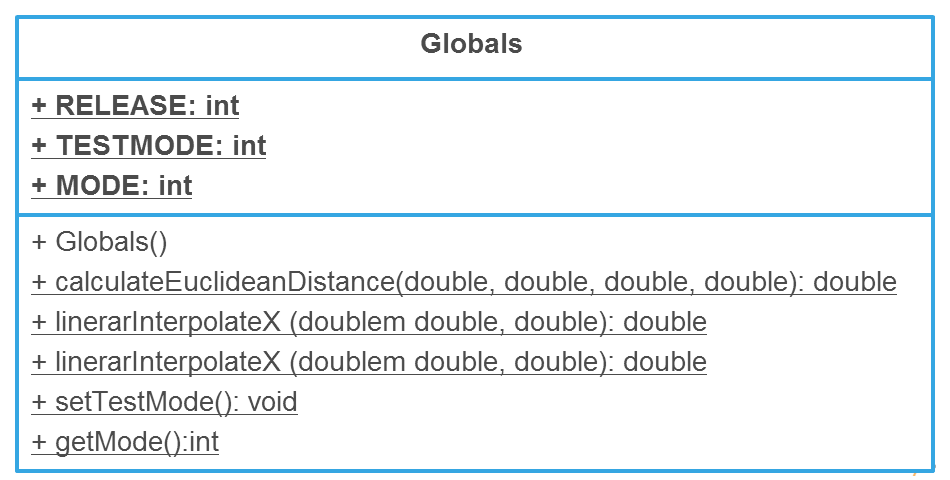
\includegraphics[scale=0.3]{Images/chapter4/gloabls}
\caption{The contents of the Utils package show in standard UML Class diagram notation}
\label{fig:utilsImp}
\end{figure}

Figure \ref{fig:utilsImp} represents the single Class contents of the Utils package. This Globals Class contains several publically avliable static variables and methods enabling application wide access. This enables the multiple packages which rely on the results of the features present to still have access whilst also reducing the amount of repeated code in the application. In addition to this, this Class also enables the execution mode to be switched from release, to test mode. When in test mode the error messages require no user response enabling the automated test process to complete more easily.

\subsection{System Interactions}

\Large WRITE THIS SECTION \normalsize

\section{Design Patterns}
\subsection{Model-View-Controller}
The current design still maintains and adheres to the Model-View-Controller(MVC) principles discussed in Appendix B, section \ref{sssec:mvc} however, the complexity of the different packages has changed both in terms of internal package structure and features provided. As designed, the author has implements an MVC compliant architecture is through the use of the Observer and Obseravle relationship using the corresponding default Java Classes. The general conecpt is implemented as defined in appendix B, section \ref{obby} slight modification have been made to the Classes representing the different components of the Observer and Observable concept.

\begin{figure}[H]
\centering
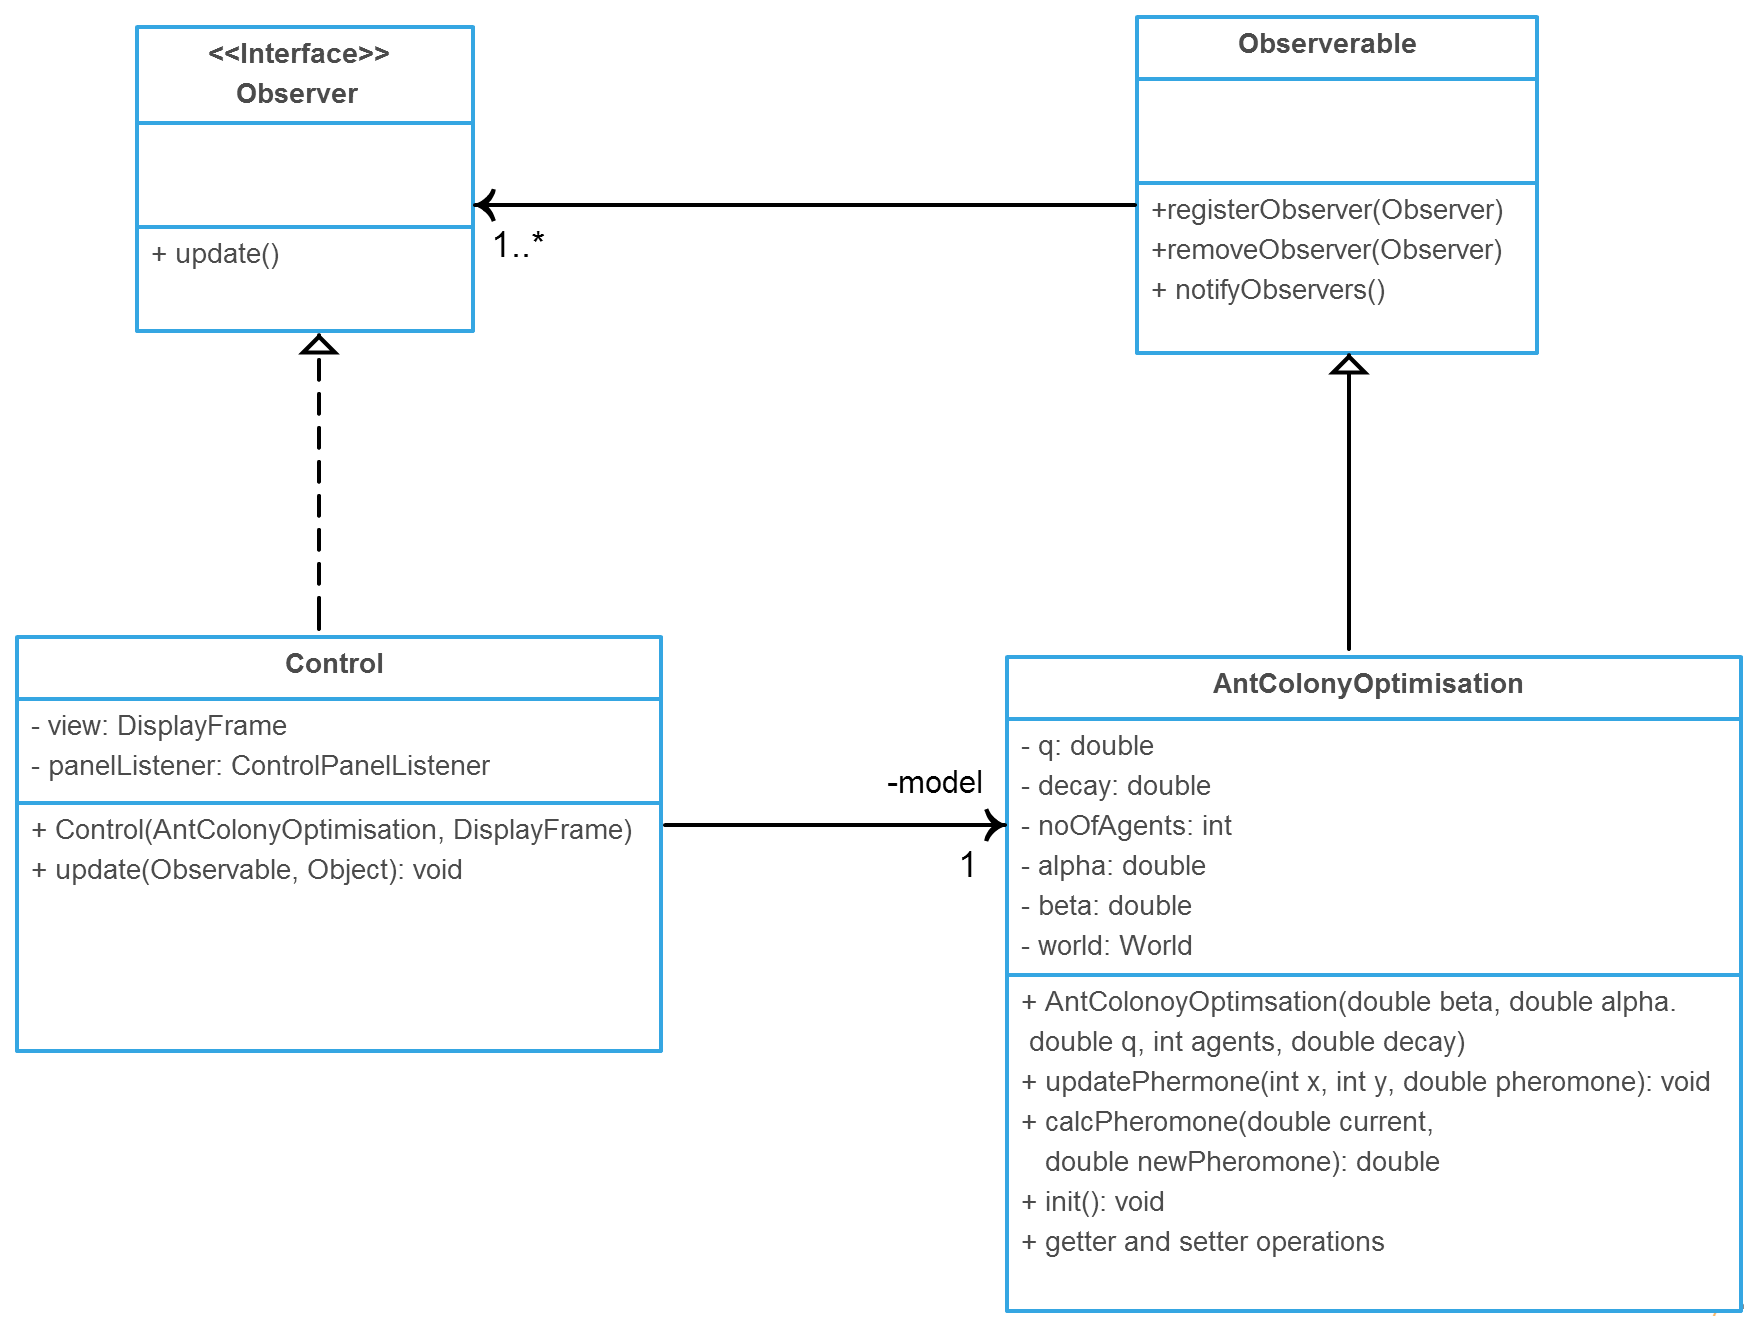
\includegraphics[width=0.9\textwidth]{Images/chapter4/observerImplemetation}
\caption{Implementation of the Observer and Observable Design pattern}
\label{fig:observableImp}
\end{figure}

Figure \ref{fig:observableImp} demonstartes how the Control Class will implement the Observer interface, which will listen to the Observable Object and determine correct actions based upon the source of update. The AntColonyOptimisation Class is as defined in section \ref{model:classdef} is the Object which is in fact Observable, and extends the Observable super Class. As the AntColonyOptimisation instance is now a subclass of Observable, it now has access to key methods such as $registerObserver()$ which allows the athor to assign the Control instance as the desiginated Observer and $notifyOberservers()$ which enables the author to dictate when updates are published, this enables the Control instance to process update notifications and notify the relevant view elements that the state of the model has changed, enabling the seperation of the view and model.

\subsection{Singleton}

Initially the author proposed that the user interface elements would implement the Singleton design pattern\cite{gof:design:singleton}, an example this proposed design can be seen in appendix B, section \ref{sssec:singleton} however, the Singleton pattern is not present in the current system architecture. The author initially implemented the main elements from the view package (see \ref{view:clss}) this caused several complications for the author. As the instance of the Singleton Object is globally accessible, difficulties arose during the application debugging. This issue happened to be more prevalent when extending the functionality provided by each of the Singleton Classes, for example the DisplayFrame Class now handles contains a wider range of functionality than initial planned. Not only did the Singleton instance make the addition of these extended features more complicated than the author intended, debugging these new features became more difficult as the global access made it harder to track the source of the bug itself. This is due the fact that it is easy to accidently interact and modify a global variable or instance, often the source of these bugs were not where the author expected and were often due to an incorrect interaction with these new extensions in a package which should not be able to access them. This was the main reason the author decided to withdraw the use of the Singleton pattern as the author felt it was much simpler to not have global access to these instances and features.

Robert Martin created idea of the Single Responsibility Principle (SRP) in 1990 \cite{SRP:site}. The general concept behind the SRP is that each logical module in the software should have one reason to change or model one specific responsibility rather than a collection of unrelated features or functions. If a module has been extended to support multiple unrelated features, the SRP states that the unrelated features should be extracted into relevant modules so that each module maintains its one responsibility. The author feels that implementing the Singleton in the proposed manner (see appendix B, section \ref{sssec:singleton}) violated the underlying concepts of the SRP. As the Singleton Class is responsible for tracking and instantiation of its one allowed instance and the functionality which the module presents. This Class now has more than one responsibility and thus breaks the SRP. The author believes the SRP should be regarded highly during development in order to produce maintainable and extendable software, thus he has opted for adhering to the SRP over the Singleton implementations. The author experimented with the idea of having extracting the functionality of the singleton Classes and the tracking of the instance of such Classes into separate system modules. Once this is done each module will have one responsibility thus, adhering to the SRP. 

Overall, the author sees the implementation of the Singleton Design pattern as more of an anti-pattern. As this is the case and to enable easier modification and future extension the implementation of any Singleton Class as initially designed has been removed. Solutions the above problems could be refactored in, but this is seen as unnecessary complexity by the author and has therefore also been omitted.

\section{User Interface}

\subsection{Main Display}

The design for the main display, which refers the general view the user will be presented and interact with remains unchanged from the initial proposal as represented in figure \ref{fig:interface}. There has been modifications to this design during the implementation phase however, these the authors flexible process (see section \ref{processSec}) and the fact that these changes were fairly trivial allowed the author to implement them without any prior design, section \ref{mainimp} displays the implemention of this design and said changes.

\subsection{Uphill Viewer}
\label{uphillview}

The uphill viewer was not an element of the user interface which was initially planned, however the addition to implement the ability for a path to represent uphill terrain called for a view to summarize which of these paths are in fact subject to this uphill modification during the given problem. This interface is a result of the contents of the UphillViewer Class (see section \ref{view:clss}).

\begin{figure}[H]
\centering
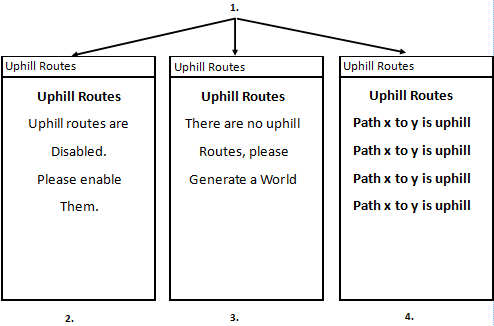
\includegraphics[scale=0.7]{Images/chapter4/uphilviews}
\caption{Abstract proposal for the uphill viewer interface representing the different states possible at runtime.}
\label{fig:uphillViewImp}
\end{figure}

\textbf{1.} in figure \ref{fig:uphillViewImp} is used to demonstrate that each possible state for the uphill viewer will be represented using the same high level container. \textbf{2.} in figure \ref{fig:uphillViewImp} is used to show the default state and content for the uphill viewer interface. This state and content is shown to the user if the uphill routes is current disabled for this problem, and prompts the user to enable them. \textbf{3.} in figure \ref{fig:uphillViewImp} is shown to the user if uphill routes are enabled, but the current world is yet to be generated. \textbf{4.} in figure \ref{fig:uphillViewImp} is shown to the user when both uphill routes are enabled for the current problem and they have been generated. The $x$ and $y$ values in this figure will be replaced with indexes of valid cities to enable to the user to understand which routes are uphill.

\subsection{City Detail Viewer}
\label{deetzlview}

The City Detail Viewer is used to summarize how many agents are at each City for the current problem. This view was not initially designed however, the author felt that this was a necessary addition and therefore designed a rough outline to how this interface is to be presented.

\begin{figure}[H]
\centering
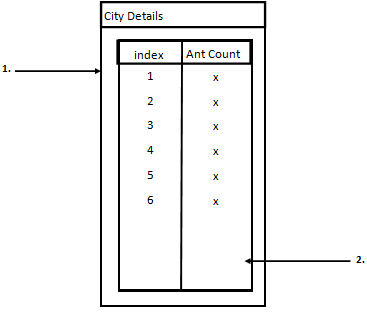
\includegraphics[scale=0.7]{Images/chapter4/citydetails}
\caption{Abstract proposal for the city detail interface.}
\label{fig:deetzViewImp}
\end{figure}

\textbf{1.} in figure \ref{fig:deetzViewImp} is showing how this view is contained in a separate container to the main display. This enables the user to move this view around as desired in order to customise the current view to their tastes. \textbf{2.} in figure \ref{fig:deetzViewImp} shows how the contents of the CityDetailView will be implemented (see section \ref{view:clss}). The number of rows will directly relate to the number of City Objects in the current problem. The $x$ values will be substituted for the correct number of ants at the corresponding city index.







\subsection{Equation Viewer}
\label{eqnlview}

\subsection{Error Feedback}

\subsubsection{Parameter Errors}

\subsubsection{File IO Errors}

\section{Algorithms}

TALK ABOUT INITIAL PROPOSED PSEUDO CODE AS WELL AS HOW ITS CHANGED, TALK ABOUT PAINITNG PSUDEO CODE AND HOW THE ADDITION ON ELITIST ANTS HAS CHANGED THE PSEUDO CODE, OR SHOW THE ELITIST ANT PSEUDO CODE SEPERATELY 

ALSO FLOWCHARTS


\chapter{Implementation PUT IN OWN FILE}

\section{User interface}
\subsection{Main Display}
\label{mainimp}
The main display represents the general interface is displayed to the user. This is where the algorithms visual representation will be presented, as well as providing the location of the user interaction elements enabling modification of the algorithms parameters. This interface is a result of the contents of the DisplayFrame Class and its contents. The design for this view is generally as described in section \ref{ssec:mainUI}, appendix B, however, there has been a slight modification to this proposed design.

\begin{figure}[H]
\centering
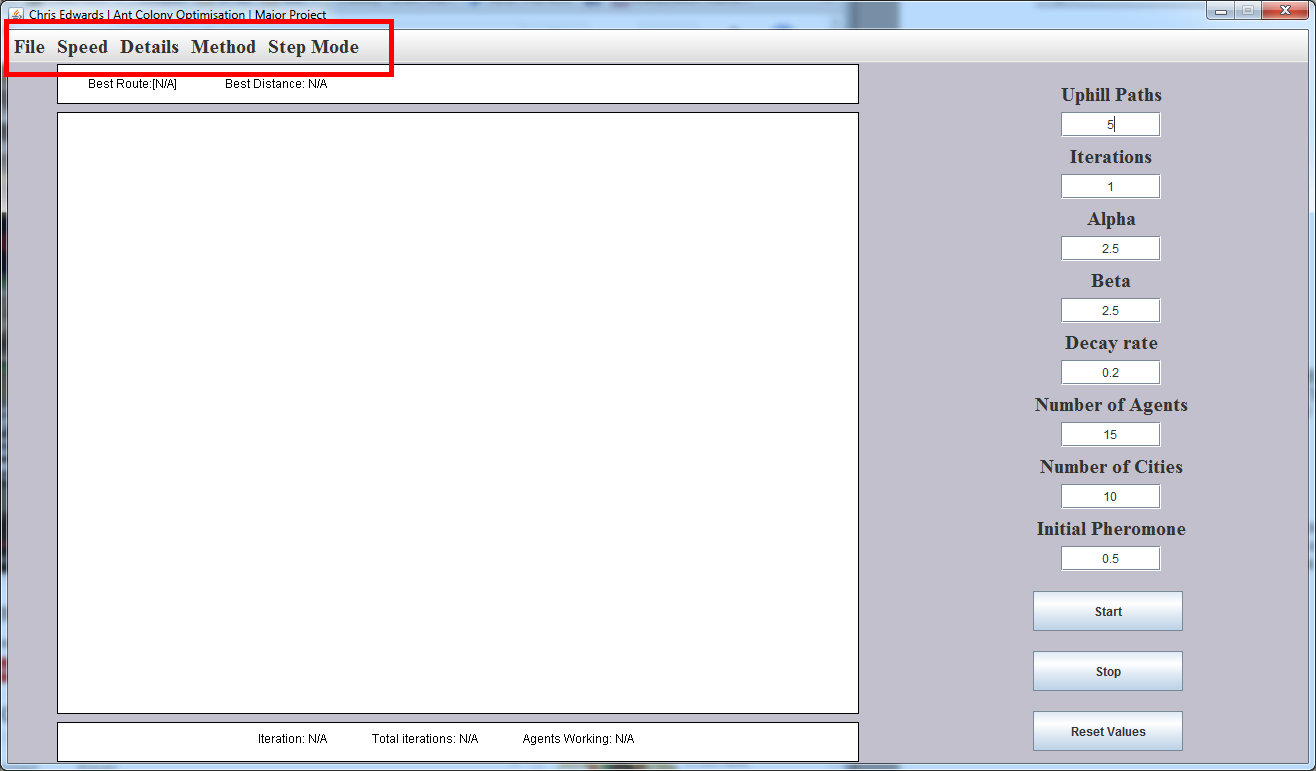
\includegraphics[scale=0.35]{Images/chapter4/displayFrame}
\caption{Implementation of the proposed user interface. The contents of the red polygon highlights the additional features not present in the initial design.}
\label{fig:displayFrameImp}
\end{figure}

The additional features highlighted by the red polygon in figure \ref{fig:displayFrameImp} represent the features which were not initially designed. These features are represented in a separate location to the control panel (right hand side of figure \ref{fig:displayFrameImp}) as there is no logical connection between the menu bar features, and the modification of the algorithm parameters. The author opted to use a menu bar to control the access to these features as the vast majority of users will recognise what a menu bar is, and understand how to interact with such elements. 

The different elements contained in this menu bar relate to general system interactions. The File option enables the user to either load, or save a configuration to a specified file. The Speed option enables the user to change the Thread speed, which will directly change the algorithms rate of execution. The Details menu is used to control access to any additional views. The views which can be access here are; the Uphill Viewer (section \ref{uphillview}), The City Detail View (section \ref{deetzlview}) and the Equation Viewer (section \ref{eqnlview}). In addition to the access of these extra views, the Detail menu also enables the user to disable and enable uphill routes \Large REFERENCE UPHILL ROUTES GENERATION ALGORITHM PSEUDO CODE \normalsize to be generated for current problem. The Method option enables the user to select the current algorithm type from a list of implement algorithm types. Currently the author has implemented a Basic Ant System and an Elitist Ant system so the user can switch between these algorithm types. The Step Mode menu enables the user to enable or disable the step mode functionality. When enabled, step mode will allow the user to step through the algorithms execution at their own pace without the application automatically solving the problem.

The implementation should look at any issues you encountered as you tried to implement your design. During the work, you might have found that elements of your design were unnecessary or overly complex; perhaps third party libraries were available that simplified some of the functions that you intended to implement. If things were easier in some areas, then how did you adapt your project to take account of your findings?

It is more likely that things were more complex than you first thought. In particular, were there any problems or difficulties that you found during implementation that you had to address? Did such problems simply delay you or were they more significant? 

You can conclude this section by reviewing the end of the implementation stage against the planned requirements. 

\chapter{Testing PUT THIS IN OWN FILE}

Detailed descriptions of every test case are definitely not what is required here. What is important is to show that you adopted a sensible strategy that was, in principle, capable of testing the system adequately even if you did not have the time to test the system fully.

Have you tested your system on �real users�? For example, if your system is supposed to solve a problem for a business, then it would be appropriate to present your approach to involve the users in the testing process and to record the results that you obtained. Depending on the level of detail, it is likely that you would put any detailed results in an appendix.

The following sections indicate some areas you might include. Other sections may be more appropriate to your project. 

\section{Overall Approach to Testing}

\section{Automated Testing}

\subsection{Unit Tests}

\subsection{User Interface Testing}

\subsection{Stress Testing}

\subsection{Other types of testing}

\section{Integration Testing}

\section{User Testing}